\documentclass[12pt,oneside]{article}
\usepackage[
    a4paper,
    top=1.8cm,
    bottom=1.7cm,
    left=2cm,
    right=2cm,
    headheight=34pt,
    headsep=8pt,
    footskip=16pt
]{geometry}

\usepackage[T1]{fontenc}
\usepackage[utf8]{inputenc}
\usepackage[spanish,es-tabla]{babel}
\usepackage{lmodern}
\usepackage{mathptmx}
\usepackage{amsmath}
\usepackage[protrusion=true,expansion=true]{microtype}
\usepackage{graphicx}
\usepackage{float}
\usepackage{caption}
\usepackage{booktabs}
\usepackage{array}
\usepackage{makecell}
\renewcommand{\theadfont}{\bfseries\footnotesize}
\usepackage{tocloft}
\usepackage{fancyhdr}
\usepackage{csquotes}
\usepackage{titlesec}
\usepackage[
    colorlinks=true,
    linkcolor=black,
    urlcolor=blue,
    citecolor=black,
    pdftitle={Análisis de respuesta de sitio para Neiva — Entrega 3},
    pdfauthor={Andrés Stiven Jaramillo Cataño, Emmel Escovitch Riaño, Laury Yocely Perea Mena}
]{hyperref}
\usepackage{xcolor}
\newcommand{\pendiente}[1]{{\color{red}\itshape [Pendiente: #1]}}
\usepackage[backend=biber,style=apa,sortcites=true]{biblatex}
\addbibresource{biblio.bib}

\setlength{\emergencystretch}{2em}
\setlength{\parindent}{0pt}
\setlength{\parskip}{3pt}
\setlength{\textfloatsep}{8pt plus 2pt minus 2pt}
\setlength{\intextsep}{8pt plus 2pt minus 2pt}
\captionsetup{font=footnotesize,skip=3pt}
\newcommand{\customtablecaption}[2]{%
    \refstepcounter{table}%
    \caption*{#1. #2}%
    \addcontentsline{lot}{table}{#1. #2}%
}
\renewcommand{\contentsname}{Índice de contenido}
\renewcommand{\listtablename}{Índice de tablas}
\renewcommand{\listfigurename}{Índice de figuras}
\AtBeginDocument{%
    \renewcommand{\contentsname}{Índice de contenido}%
    \renewcommand{\listtablename}{Índice de tablas}%
    \renewcommand{\listfigurename}{Índice de figuras}%
}
\setlength{\parskip}{0pt}
\setlength{\cftbeforetoctitleskip}{0pt}
\setlength{\cftaftertoctitleskip}{4pt}
\setlength{\cftbeforelottitleskip}{8pt}
\setlength{\cftafterlottitleskip}{4pt}
\setlength{\cftbeforeloftitleskip}{8pt}
\setlength{\cftafterloftitleskip}{4pt}
\setlength{\cftbeforesecskip}{0pt}
\setlength{\cftbeforetabskip}{0pt}
\setlength{\cftbeforefigskip}{0pt}

\titleformat{\section}
    {\normalfont\large\bfseries}
    {\thesection.}
    {0.5em}
    {}
\titlespacing*{\section}{0pt}{10pt}{4pt}

\pagestyle{fancy}
\fancyhf{}
\fancyhead[L]{
\includegraphics[height=0.85cm]{../figuras/Logo_encabezado.png}}
\fancyhead[R]{\footnotesize Ingeniería Sismo-Geotécnica}
\fancyfoot[C]{\footnotesize Página \thepage}
\renewcommand{\headrulewidth}{0.4pt}
\renewcommand{\footrulewidth}{0pt}

\begin{document}
\decimalpoint

\begin{titlepage}
    \centering
    \thispagestyle{empty}
    \setlength{\parskip}{0pt}
    \vspace*{0.3cm}
    
\includegraphics[width=0.20\textwidth]{../figuras/Logo_1.png}\par

    \vspace{2.1cm}
    {\LARGE\bfseries Análisis de Respuesta de Sitio\\[6pt]
    para un Perfil de Suelo en Neiva\par}
    \vspace{0.8cm}
    {\large\bfseries Tercera entrega\par}
    \vspace{1.3cm}
    {\large\bfseries Ingeniería Sismo-Geotécnica\par}

    \vspace{1.7cm}
    {\large\bfseries Elaborado por:\par}
    \vspace{8pt}
    {\large Andrés Stiven Jaramillo Cataño\\[4pt]
    Emmel Escovitch Riaño\\[4pt]
    Laury Yocely Perea Mena\par}

    \vspace{0.9cm}
    {\large\bfseries Docente:\par}
    \vspace{8pt}
    {\large Andrés Felipe Serna Vazquez\par}

    \vfill
    {\large Universidad Nacional de Colombia\\[4pt]
    Sede Medellín\\[4pt]
    Facultad de Minas\\[4pt]
    Departamento de Ingeniería Civil\\[4pt]
    \pendiente{Fecha de entrega}\par}
    \vspace{0.3cm}
\end{titlepage}

\pagenumbering{roman}
\tableofcontents
\listoftables
\listoffigures
\clearpage
\setlength{\parskip}{3pt}
\pagenumbering{arabic}

\section{Introducción y metodología}

Este informe evalúa la respuesta sísmica de un perfil de suelo de 30 m en
Neiva, apoyado sobre roca. El movimiento en roca es el obtenido en la
Entrega 2: PGA de 475 años de 0.196 $g$ y espectro de aceleración en roca
con meseta de 0.481 $g$. \pendiente{Confirmar si la entrada en roca se
define con el PGA (0.196 $g$) o con el $A_a$ equivalente (0.19).}

El trabajo sigue los siete puntos del enunciado:
\begin{enumerate}
    \item \textbf{Perfil estratigráfico:} clasificación y propiedades
    dinámicas de cada estrato, a partir de los ensayos de campo y laboratorio.
    \item \textbf{Curvas de degradación:} $G/G_{\max}$ y amortiguamiento
    contra deformación cortante para cada estrato.
    \item \textbf{Análisis modal de Zeevaert:} desplazamientos y módulo de
    rigidez contra profundidad \parencite{zeevaert1983}.
    \item \textbf{Sismos de análisis:} tres registros de fuente cercana,
    intermedia y lejana.
    \item \textbf{Análisis en DEEPSOIL:} desplazamientos y módulo de rigidez
    contra profundidad, comparados con Zeevaert \parencite{deepsoil2020}.
    \item \textbf{Espectro en superficie:} espectro de DEEPSOIL comparado con
    el de la NSR-10 \parencite{nsr10}.
    \item \textbf{Licuación:} potencial de licuación con el nivel freático en
    superficie.
\end{enumerate}

\section{Punto 1: perfil estratigráfico}

\subsection{Ensayos disponibles}

Se cuenta con un sondeo (P-1) de 30 m con los ensayos de la
Tabla~\ref{tab:ensayos}.

\begin{table}[H]
\centering
\customtablecaption{Tabla 1}{Ensayos de campo y laboratorio del sondeo P-1.}
\label{tab:ensayos}
\footnotesize
\renewcommand{\arraystretch}{1.25}
\begin{tabular}{|l|>{\raggedright\arraybackslash}p{2.6cm}|>{\raggedright\arraybackslash}p{4.2cm}|}
\hline
\thead{Ensayo} & \thead{Profundidades\\(m)} & \thead{Uso} \\
\hline
Down hole ($V_p$ y $V_s$, 40 canales) & 1 a 40 & $V_s$, $V_p$, $\nu$ y $G_{\max}$ \\ \hline
Humedad, granulometría y límites & 3, 6, 12, 16, 22, 26 y 30 & Clasificación USCS \\ \hline
Triaxial estático CU & 4 y 28 & $\phi'$, $c'$ y $\gamma_h$ \\ \hline
Triaxial cíclico (ASTM D3999) & 5 & Curva de la arena \\ \hline
Columna resonante (ASTM D4015) & 10 y 20 & Curvas de arena y arcilla \\ \hline
\end{tabular}
\end{table}
\subsection{Clasificación USCS}

Se ven dos estratos claramente diferentes (Tabla~\ref{tab:clasificacion}):
arriba una arena con grava y limo (SP-SM) y abajo una arcilla. La arcilla es de
baja plasticidad (CL) y se vuelve más plástica a medida que se baja (LL de 26
a 50\%); la muestra de 30 m ya clasifica como CH.

\begin{table}[H]
\centering
\customtablecaption{Tabla 2}{Clasificación de las muestras del sondeo P-1.}
\label{tab:clasificacion}
\footnotesize
\renewcommand{\arraystretch}{1.25}
\begin{tabular}{|l|c|c|c|c|c|c|c|c|l|}
\hline
\thead{Muestra} & \thead{Prof.\\(m)} & \thead{$w$\\(\%)} & \thead{Grava\\(\%)} & \thead{Arena\\(\%)} & \thead{Finos\\(\%)} & \thead{LL\\(\%)} & \thead{LP\\(\%)} & \thead{IP\\(\%)} & \thead{USCS} \\
\hline
P1-M3 & 3 & 23.4 & 47.1 & 43.3 & 9.6 & 29 & 23 & 6 & SP-SM \\ \hline
P1-M6 & 6 & 21.9 & 37.1 & 51.9 & 11.0 & 29 & 24 & 5 & SP-SM \\ \hline
P1-M12 & 12 & 20.4 & 47.1 & 43.3 & 9.6 & 29 & 23 & 6 & SP-SM \\ \hline
P1-M16 & 16 & 22.4 & 0.0 & 16.4 & 83.6 & 26 & 15 & 11 & CL \\ \hline
P1-M22 & 22 & 36.6 & 0.0 & 3.7 & 96.3 & 36 & 20 & 16 & CL \\ \hline
P1-M26 & 26 & 27.7 & 0.0 & 6.6 & 93.4 & 38 & 21 & 17 & CL \\ \hline
P1-M30 & 30 & 24.1 & 0.0 & 6.5 & 93.5 & 50 & 23 & 27 & CH \\ \hline
\end{tabular}
\end{table}
\pendiente{Revisar con el profesor: la muestra P1-M12 tiene la misma
granulometría y los mismos límites que P1-M3, y en ambas la grava (47.1\%)
supera a la arena (43.3\%), por lo que la USCS daría GP-GM o GW-GM.}

\subsection{Consistencia a partir de los límites de Atterberg}

Para no quedarnos solo con el IP, se calculan también el índice de liquidez,
$I_L=(w-LP)/IP$, y el de consistencia, $I_C=(LL-w)/IP$
(Tabla~\ref{tab:atterberg}).

\begin{table}[H]
\centering
\customtablecaption{Tabla 3}{Índices de liquidez y consistencia.}
\label{tab:atterberg}
\footnotesize
\renewcommand{\arraystretch}{1.25}
\begin{tabular}{|l|c|c|c|l|c|c|>{\raggedright\arraybackslash}p{2.1cm}|>{\raggedright\arraybackslash}p{1.5cm}|>{\raggedright\arraybackslash}p{2.3cm}|}
\hline
\thead{Muestra} & \thead{Prof.\\(m)} & \thead{$w$\\(\%)} & \thead{IP\\(\%)} & \thead{USCS} & \thead{$I_L$} & \thead{$I_C$} & \thead{Consist.\\según $I_L$} & \thead{Consist.\\según $I_C$} & \thead{Plasticidad} \\
\hline
P1-M3 & 3 & 23.4 & 6 & SP-SM & 0.07 & 0.93 & Firme & Rígido & Poco plástico \\ \hline
P1-M6 & 6 & 21.9 & 5 & SP-SM & -0.42 & 1.42 & Semisólido o sólido & Duro & Poco plástico \\ \hline
P1-M12 & 12 & 20.4 & 6 & SP-SM & -0.43 & 1.43 & Semisólido o sólido & Duro & Poco plástico \\ \hline
P1-M16 & 16 & 22.4 & 11 & CL & 0.67 & 0.33 & Blando & Blando & Medianamente plástico \\ \hline
P1-M22 & 22 & 36.6 & 16 & CL & 1.04 & -0.04 & Líquido & Muy blando & Medianamente plástico \\ \hline
P1-M26 & 26 & 27.7 & 17 & CL & 0.39 & 0.61 & Firme & Medio & Medianamente plástico \\ \hline
P1-M30 & 30 & 24.1 & 27 & CH & 0.04 & 0.96 & Firme & Rígido & Altamente plástico \\ \hline
\end{tabular}
\end{table}
\begin{itemize}
    \item \textbf{Estrato 1 (arena):} es poco plástica y de firme a dura. Como
    es un suelo granular, lo que manda en su comportamiento es la fricción y
    no los finos.
    \item \textbf{Estrato 2 (arcilla):} la plasticidad sube con la
    profundidad, de media a alta. Entre 16 y 22 m es blanda; a 22 m la humedad
    (36.6\%) incluso supera el límite líquido. Hacia el fondo se vuelve más
    firme.
\end{itemize}

\subsection{Resistencia a partir del triaxial estático CU}

Se hicieron dos triaxiales CU, uno en cada estrato (Tabla~\ref{tab:cu}). El
criterio de falla fue el máximo esfuerzo desviador.

\begin{table}[H]
\centering
\customtablecaption{Tabla 4}{Parámetros de resistencia del triaxial CU.}
\label{tab:cu}
\footnotesize
\renewcommand{\arraystretch}{1.25}
\begin{tabular}{|l|c|c|c|c|}
\hline
\thead{Estrato} & \thead{Prof.\\(m)} & \thead{$\gamma_h$\\(kN/m$^3$)} & \thead{$\phi'$\\(°)} & \thead{$c'$\\(kPa)} \\
\hline
E1 (arena) & 4 & 18.2 & 18 & 0 \\ \hline
E2 (arcilla) & 28 & 18.1 & 1 & 69 \\ \hline
\end{tabular}
\end{table}
La arena no tiene cohesión, como es de esperar en un suelo granular. La
arcilla tiene cohesión y casi nada de fricción, así que su resistencia es
prácticamente la no drenada.

\subsection{Parámetros dinámicos}

\subsubsection{Ensayo Down Hole}

El down hole tiene 40 geófonos, uno por metro, y la fuente está en superficie
a 3 m del pozo. Para la onda P se golpea en vertical y para la onda S se dan
dos golpes horizontales en sentidos contrarios (X y Y). Las Figuras~\ref{fig:dh_p}
y~\ref{fig:dh_s} muestran los registros, con la llegada leída en cada canal.

\begin{figure}[H]
    \centering
    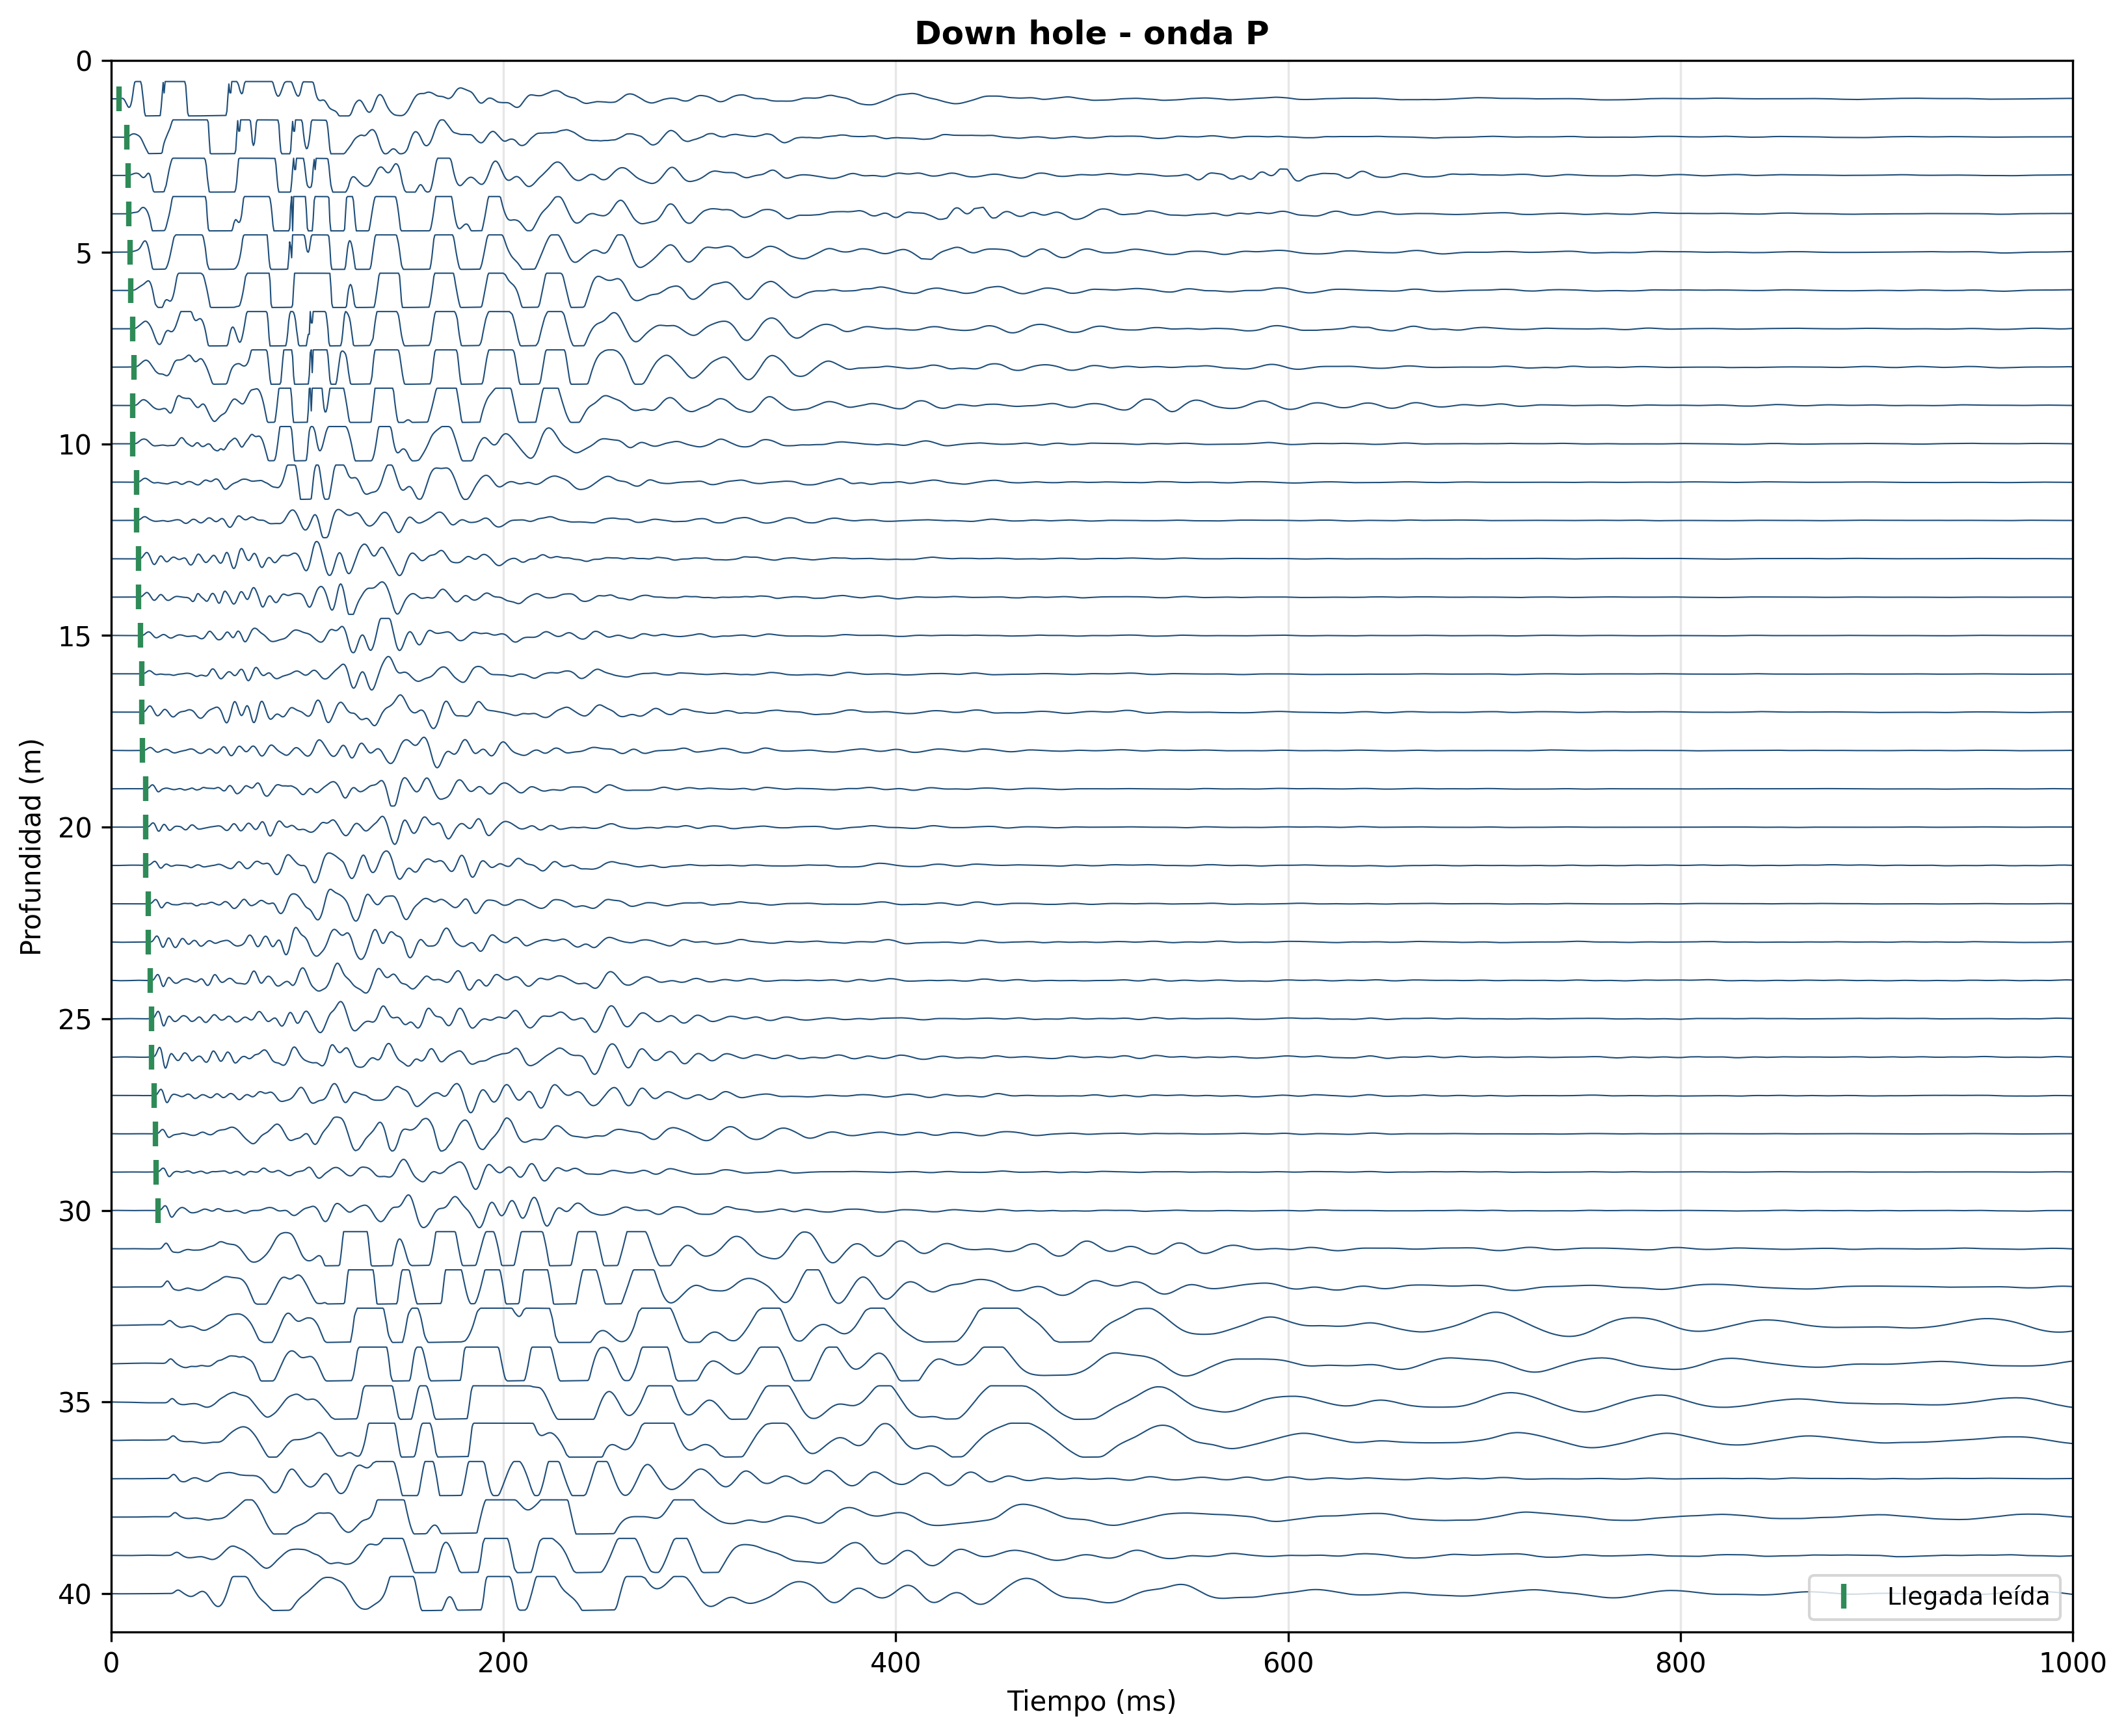
\includegraphics[width=0.9\linewidth]{../figuras/downhole_registros_p.png}
    \caption{Down hole: onda P.}
    \label{fig:dh_p}
\end{figure}

\begin{figure}[H]
    \centering
    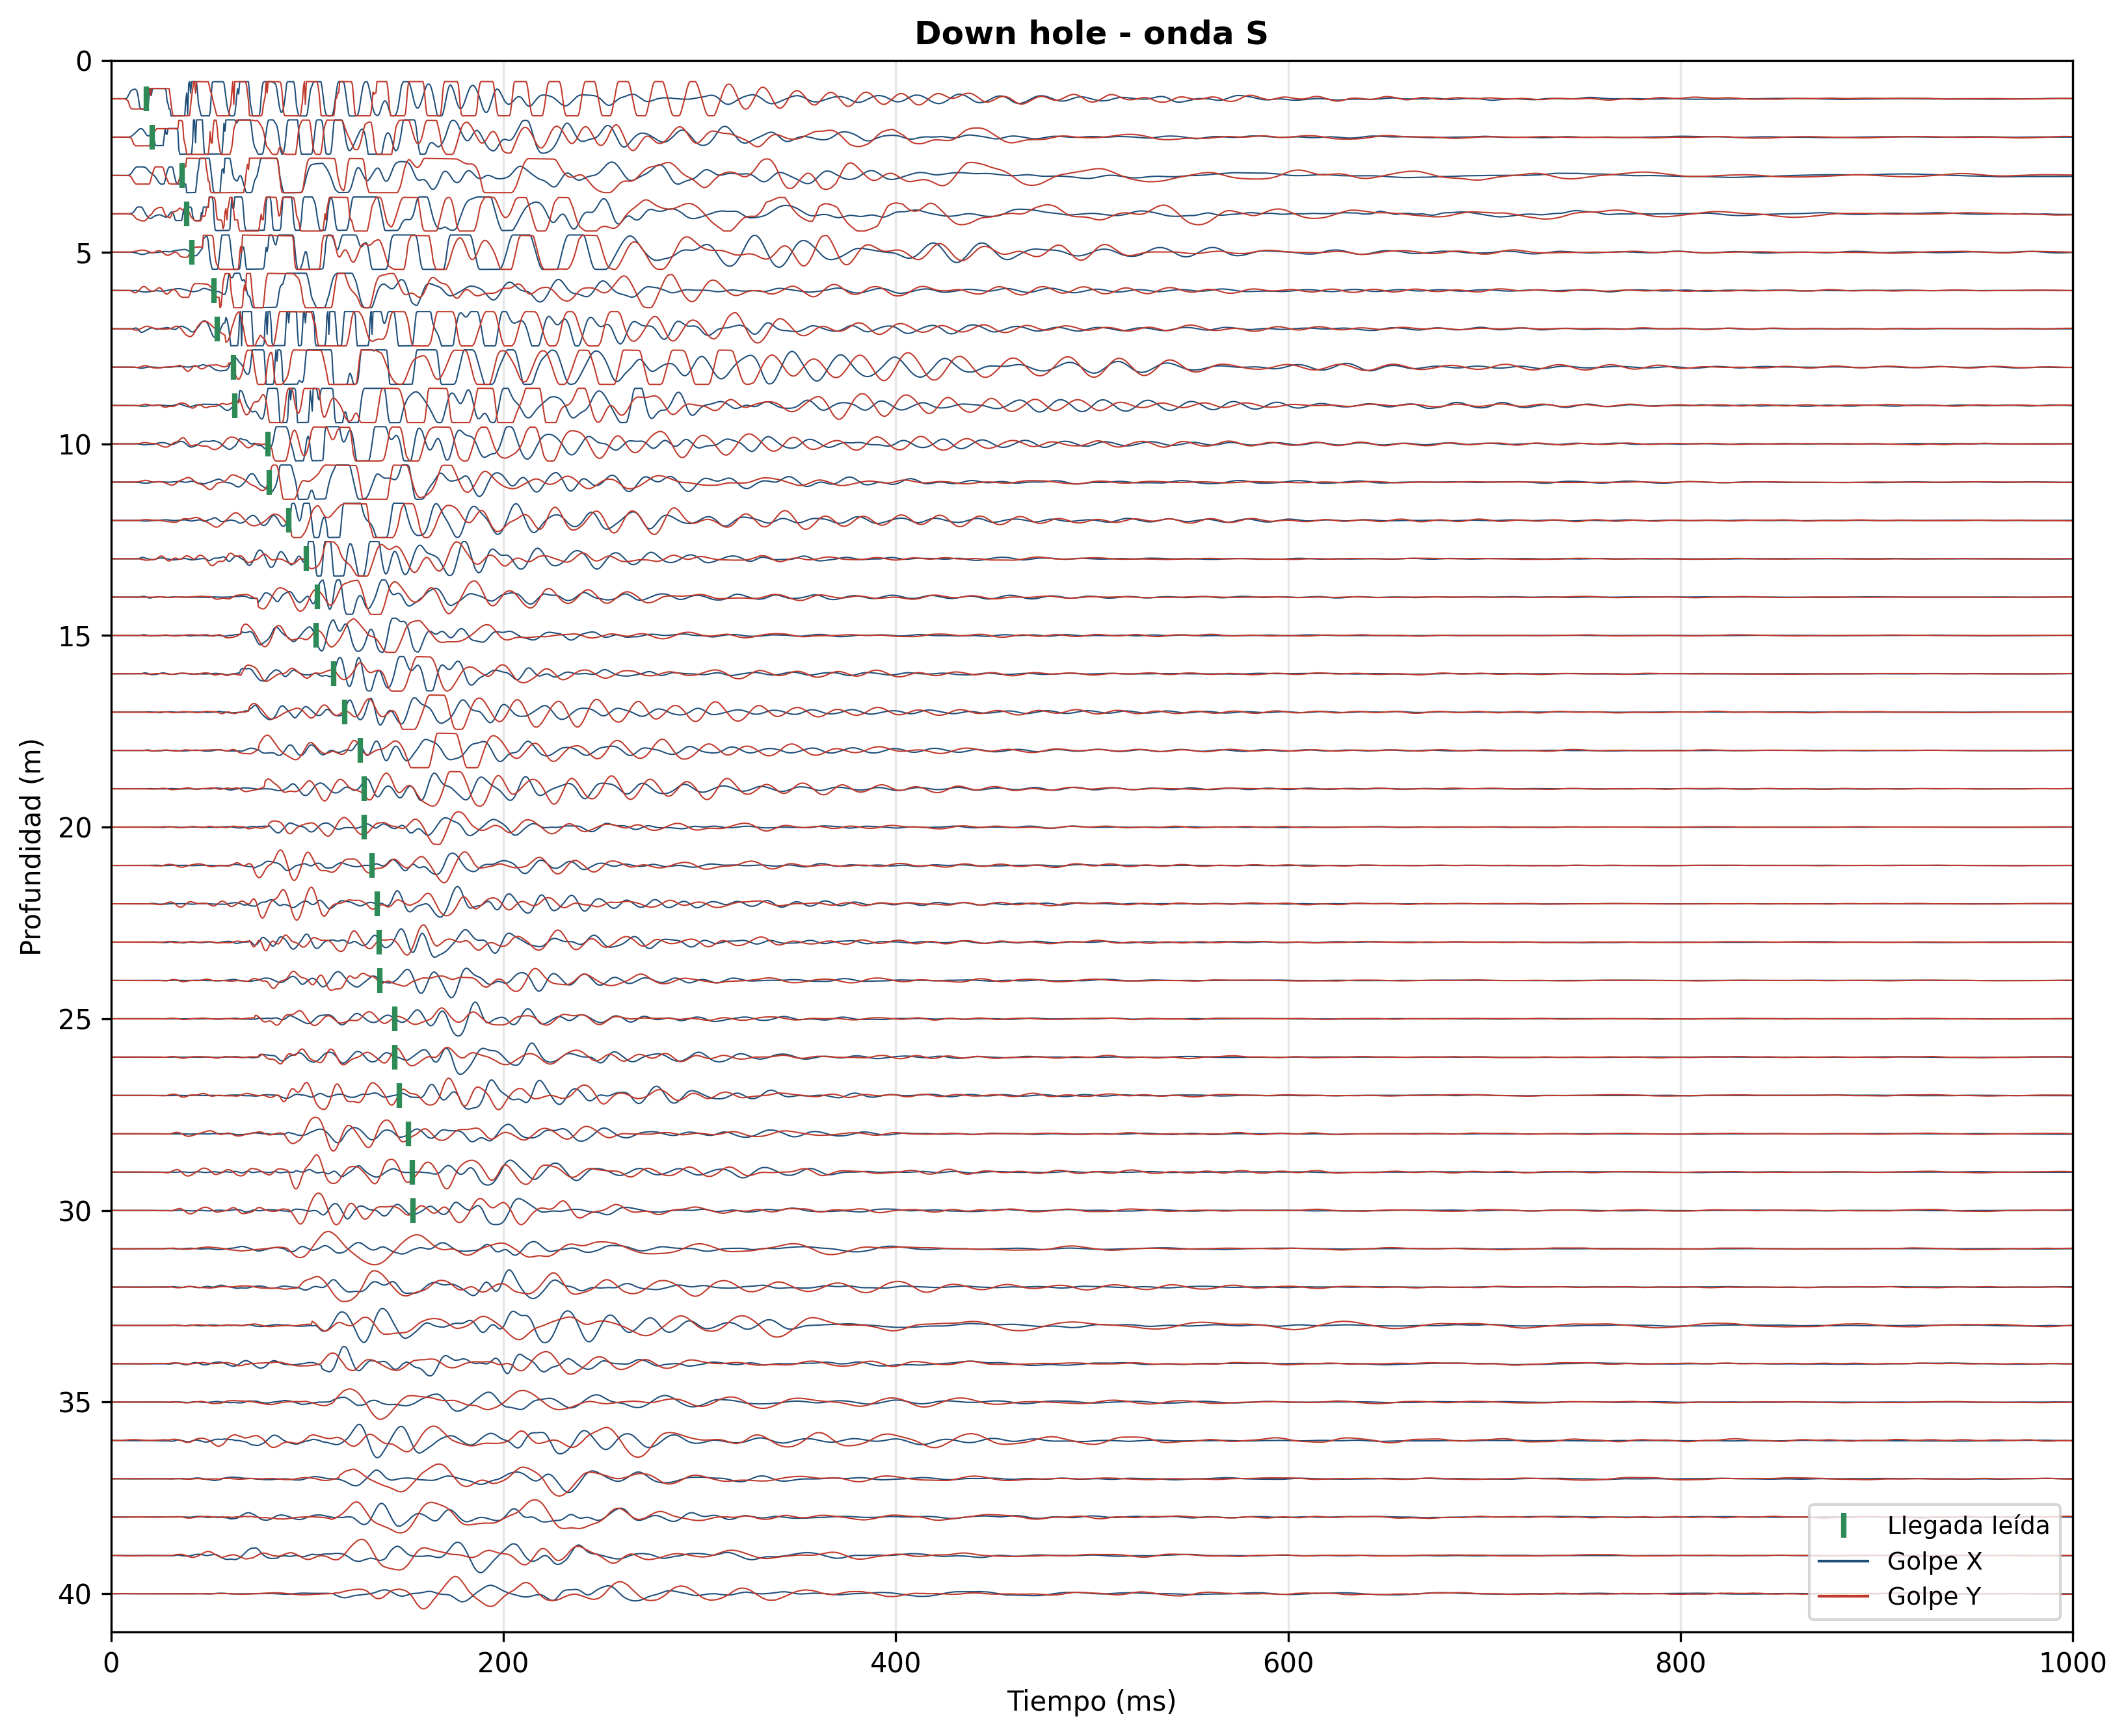
\includegraphics[width=0.9\linewidth]{../figuras/downhole_registros_s.png}
    \caption{Down hole: onda S.}
    \label{fig:dh_s}
\end{figure}

La llegada de la onda P se leyó en el primer quiebre de cada registro
\parencite{astmD7400}, y la de la onda S donde los golpes X y Y se separan en
espejo. Como la fuente no está sobre el pozo, cada tiempo se pasa a vertical
con $t_z=t\,z/\sqrt{z^2+3^2}$, y la velocidad sale de la pendiente de $t_z$
contra la profundidad. En la arena las llegadas son claras y se usan tres
rectas; en la arcilla la llegada no se ve tan clara canal por canal, así que
se usa una sola recta con los 14 canales para que los errores de lectura se
compensen. Los dos primeros metros no se usan porque están muy cerca de la
fuente. Con las velocidades se calculan el coeficiente de Poisson
$\nu$ y el módulo cortante $G_{\max}=\rho V_s^2$ de cada estrato
(Tabla~\ref{tab:perfil}). Para $\rho$ se usa el peso unitario promedio de las
muestras de cada estrato (Tabla~\ref{tab:gamma}). En los triaxiales CU el
peso unitario viene directo en los resultados; en el triaxial cíclico y en la
columna resonante el ensayo da la densidad húmeda, y se pasa a peso unitario
con $\gamma_h=\rho_h\,g$. Por ejemplo, a 5 m: $\gamma_h=1.891\ \text{g/cm}^3
\times9.81=18.55$ kN/m$^3$.

\begin{table}[H]
\centering
\customtablecaption{Tabla 5}{Peso unitario de las muestras.}
\label{tab:gamma}
\footnotesize
\renewcommand{\arraystretch}{1.25}
\begin{tabular}{|c|c|l|c|}
\hline
\thead{Estrato} & \thead{Prof.\\(m)} & \thead{Ensayo} & \thead{$\gamma_h$\\(kN/m$^3$)} \\
\hline
1 & 4 & Triaxial CU & 18.20 \\ \hline
1 & 5 & Triaxial cíclico & 18.55 \\ \hline
1 & 10 & Columna resonante & 18.91 \\ \hline
\textbf{Promedio estrato 1} & & & \textbf{18.6} \\ \hline
2 & 20 & Columna resonante & 19.28 \\ \hline
2 & 28 & Triaxial CU & 18.10 \\ \hline
\textbf{Promedio estrato 2} & & & \textbf{18.7} \\ \hline
\end{tabular}
\end{table}
\begin{table}[H]
\centering
\customtablecaption{Tabla 6}{Propiedades de los estratos.}
\label{tab:perfil}
\footnotesize
\renewcommand{\arraystretch}{1.25}
\begin{tabular}{|c|c|c|c|c|c|c|c|}
\hline
\thead{Estrato} & \thead{Espesor\\(m)} & \thead{$V_p$\\(m/s)} & \thead{$V_s$\\(m/s)} & \thead{$\nu$} & \thead{$\gamma_h$\\(kN/m$^3$)} & \thead{$\rho$\\(kg/m$^3$)} & \thead{$G_{\max}$\\(MPa)} \\
\hline
1 & 16.5 & 1\,414 & 151 & 0.494 & 18.6 & 1\,896 & 43.1 \\ \hline
2 & 13.5 & 1\,577 & 380 & 0.469 & 18.7 & 1\,906 & 275.7 \\ \hline
\end{tabular}
\end{table}
Como $\nu$ está muy cerca de 0.5 y $V_p$ es alta, el suelo está saturado y
el nivel freático está cerca de la superficie. El perfil de $V_s$ obtenido es muy
parecido al de la gráfica de referencia del enunciado
(Figura~\ref{fig:perfil}).

\subsubsection{Triaxial cíclico}

Se hizo a una muestra de 5 m de profundidad (P1-M5), que está en el estrato 1,
con un confinamiento de 200 kPa (Tabla~\ref{tab:tc}).

\begin{table}[H]
\centering
\customtablecaption{Tabla 7}{Resultados del triaxial cíclico, muestra P1-M5 (5 m).}
\label{tab:tc}
\footnotesize
\renewcommand{\arraystretch}{1.25}
\begin{tabular}{|c|c|c|c|c|c|}
\hline
\thead{Ensayo} & \thead{$\gamma$\\(\%)} & \thead{$D$\\(\%)} & \thead{$E$\\(kPa)} & \thead{$G$\\(kPa)} & \thead{$\tau$\\(kPa)} \\
\hline
1 & 0.1 & 3.65 & 85\,906.6 & 31\,817.2 & 31.8 \\ \hline
2 & 0.2 & 6.00 & 71\,226.3 & 26\,380.1 & 52.8 \\ \hline
3 & 0.5 & 9.80 & 47\,846.7 & 17\,721.0 & 88.6 \\ \hline
4 & 1 & 12.30 & 30\,447.9 & 11\,277.0 & 112.8 \\ \hline
5 & 2 & 14.30 & 17\,398.8 & 6\,444.0 & 128.9 \\ \hline
6 & 5 & 15.80 & 8\,155.7 & 3\,020.6 & 151.0 \\ \hline
7 & 10 & 16.50 & 3\,806.0 & 1\,409.6 & 141.0 \\ \hline
\end{tabular}
\end{table}
\subsubsection{Columna resonante}

Se hicieron dos ensayos, uno en cada estrato: a 10 m (P1-M10) con 200 kPa
de confinamiento y a 20 m (P1-M20) con 400 kPa (Tablas~\ref{tab:cr10}
y~\ref{tab:cr20}).

\begin{table}[H]
\centering
\customtablecaption{Tabla 8}{Resultados de la columna resonante, muestra P1-M10 (10 m).}
\label{tab:cr10}
\footnotesize
\renewcommand{\arraystretch}{1.25}
\begin{tabular}{|c|c|c|c|c|c|}
\hline
\thead{Ensayo} & \thead{$f_r$\\(Hz)} & \thead{Torque\\(N$\cdot$m)} & \thead{$\gamma$\\(\%)} & \thead{$G$\\(MPa)} & \thead{$D$\\(\%)} \\
\hline
1 & 64 & 0.02 & 0.002 & 40.07 & 0.25 \\ \hline
2 & 62 & 0.04 & 0.005 & 39.87 & 0.40 \\ \hline
3 & 60 & 0.05 & 0.01 & 39.27 & 0.50 \\ \hline
4 & 58 & 0.06 & 0.02 & 38.26 & 0.95 \\ \hline
5 & 56 & 0.07 & 0.05 & 35.64 & 2.05 \\ \hline
\end{tabular}
\end{table}
\begin{table}[H]
\centering
\customtablecaption{Tabla 9}{Resultados de la columna resonante, muestra P1-M20 (20 m).}
\label{tab:cr20}
\footnotesize
\renewcommand{\arraystretch}{1.25}
\begin{tabular}{|c|c|c|c|c|c|}
\hline
\thead{Ensayo} & \thead{$f_r$\\(Hz)} & \thead{Torque\\(N$\cdot$m)} & \thead{$\gamma$\\(\%)} & \thead{$G$\\(MPa)} & \thead{$D$\\(\%)} \\
\hline
1 & 60 & 0.05 & 0.002 & 264.37 & 0.02 \\ \hline
2 & 58 & 0.07 & 0.005 & 263.04 & 0.06 \\ \hline
3 & 56 & 0.09 & 0.01 & 259.05 & 0.18 \\ \hline
4 & 54 & 0.10 & 0.02 & 255.07 & 0.35 \\ \hline
5 & 52 & 0.11 & 0.05 & 240.45 & 0.90 \\ \hline
\end{tabular}
\end{table}
\subsection{Perfil adoptado}

El perfil tiene dos estratos (Figura~\ref{fig:perfil}): una arena con grava y
limo de 16.5 m y debajo una arcilla más rígida de 13.5 m. La muestra de 30 m
sale CH, pero está justo en el límite con CL (LL $=50\%$) y su $V_s$ es igual
al del resto de la arcilla, así que se deja en el mismo estrato.

La velocidad media de onda cortante en los 30 m superiores es
\begin{equation*}
\bar{V}_s=\frac{\sum d_i}{\sum d_i/V_{si}}
=\frac{30}{\frac{16.5}{150.8}+\frac{13.5}{380.3}}
\approx207\ \text{m/s},
\end{equation*}
por lo que el perfil es tipo D según la NSR-10 (entre 180 y 360 m/s).

\begin{figure}[H]
    \centering
    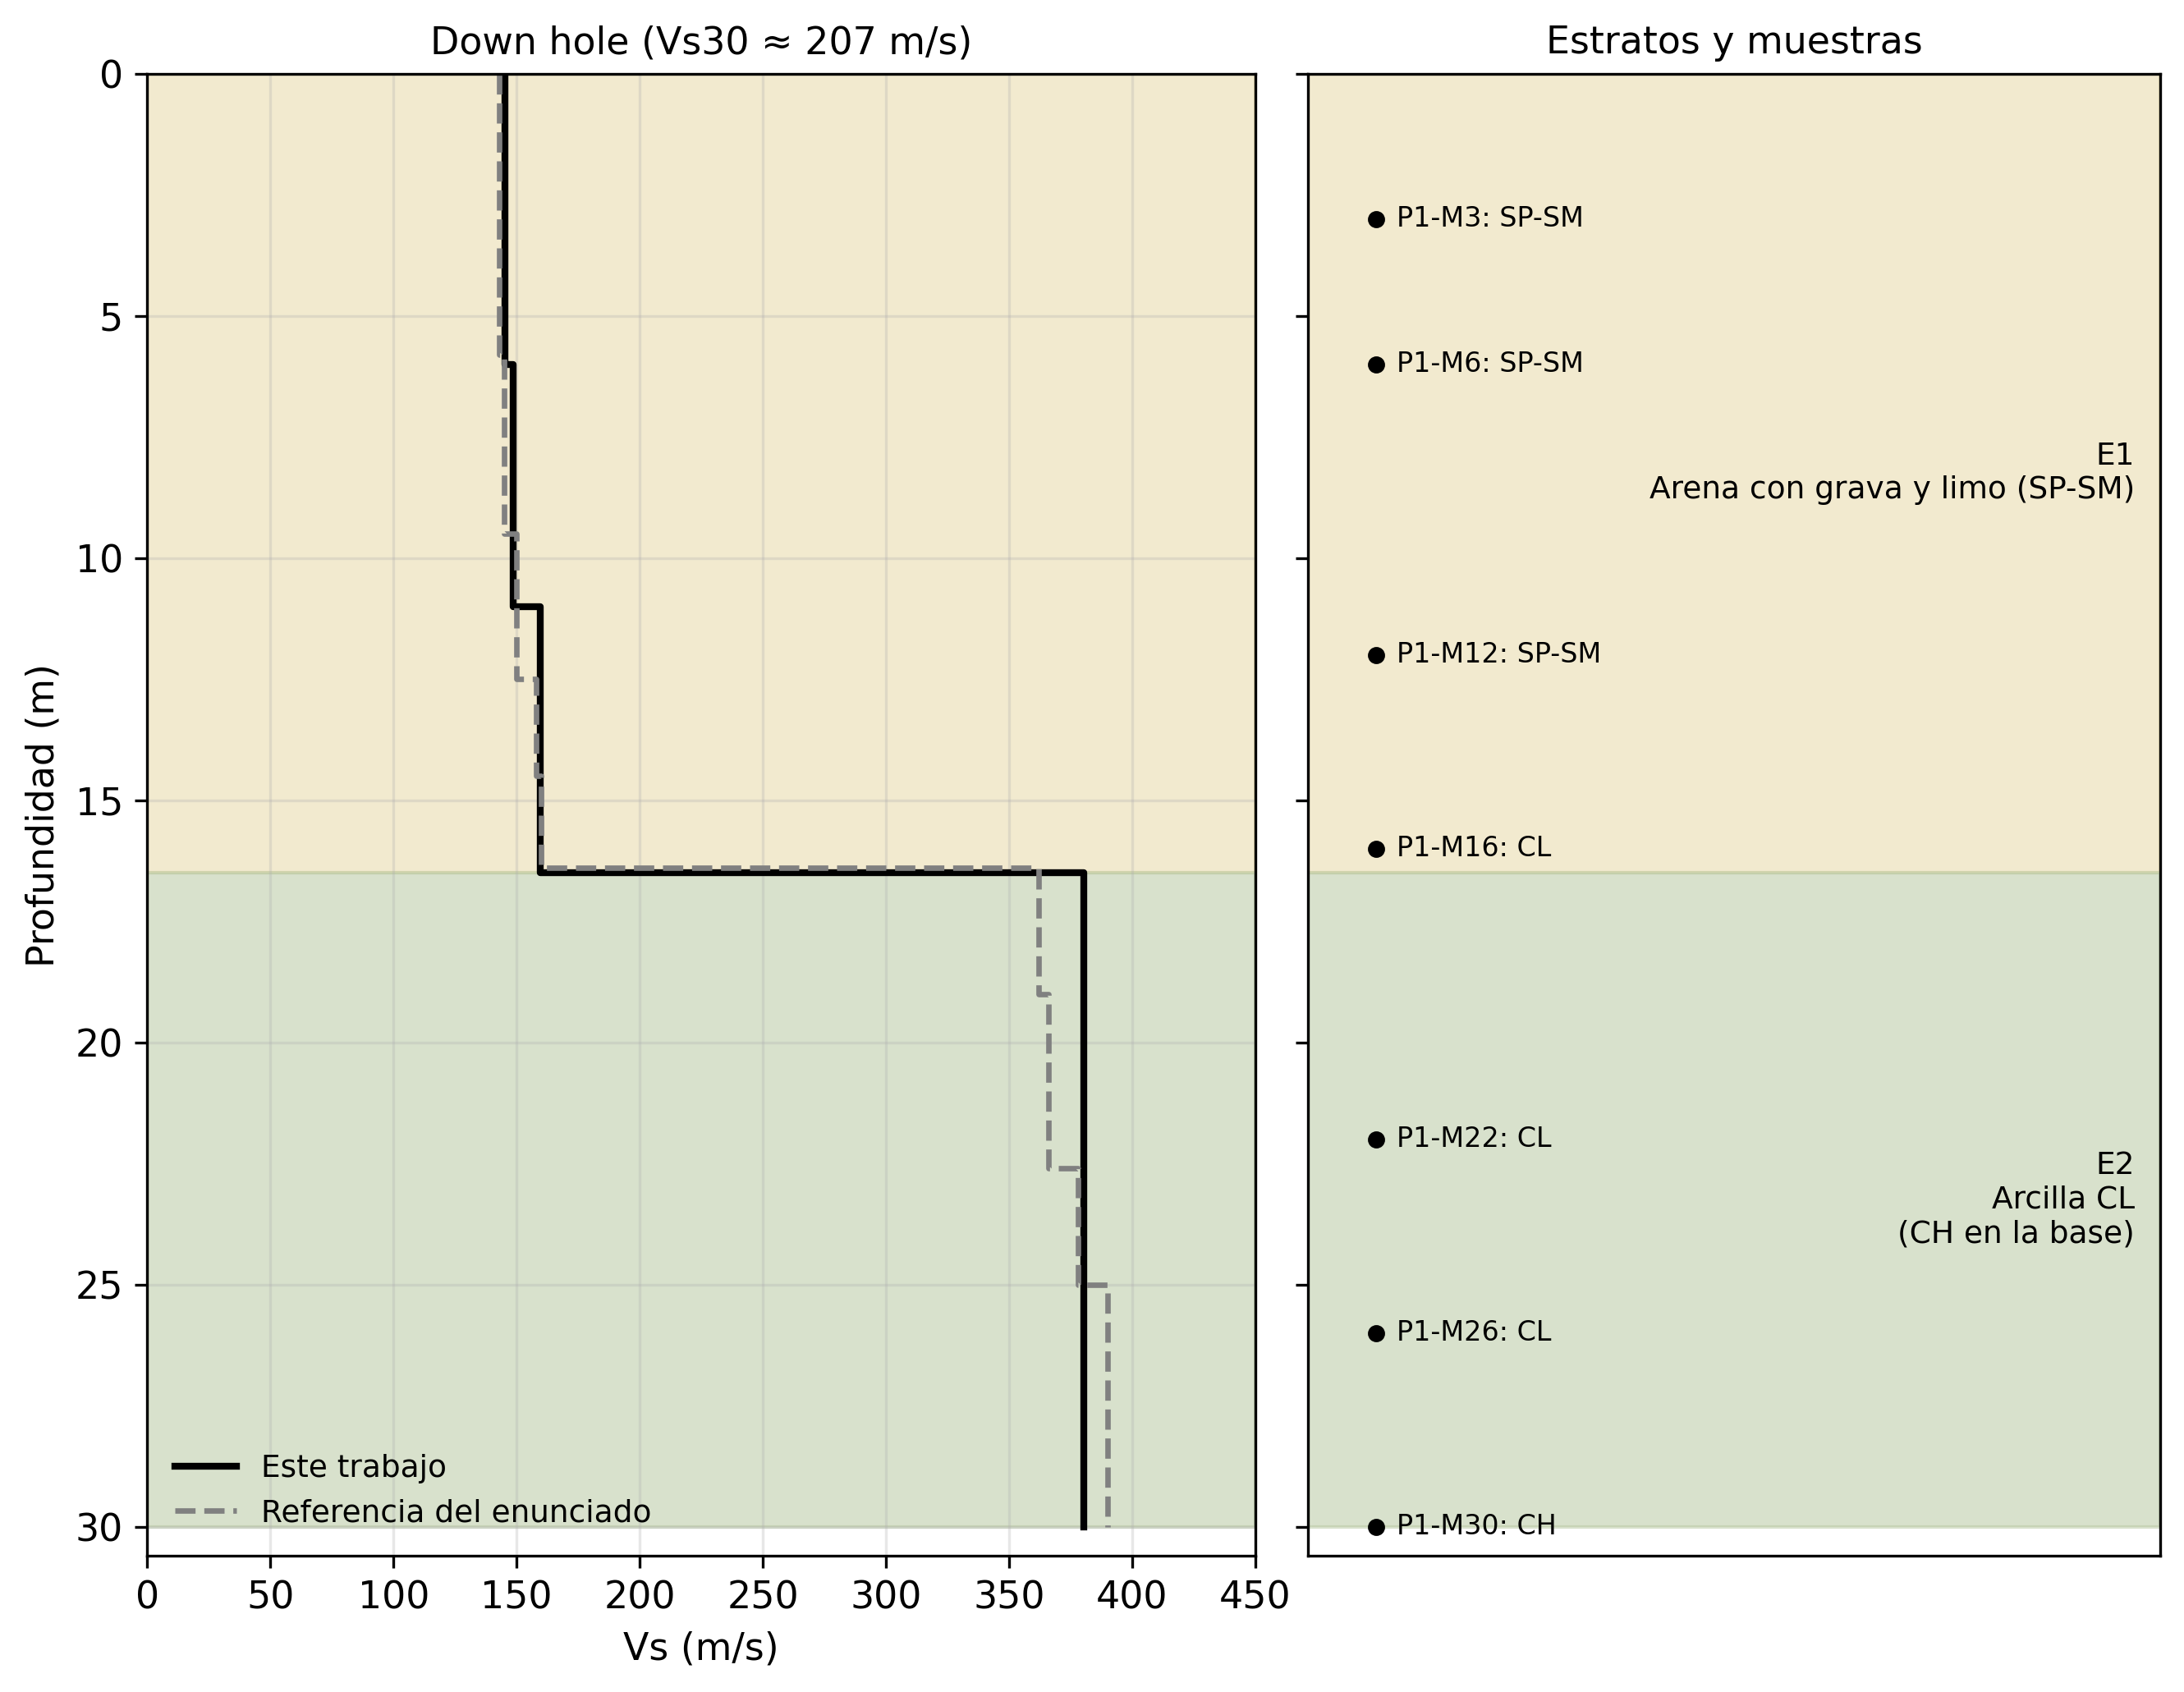
\includegraphics[width=0.72\linewidth]{../figuras/perfil_estratigrafico_p1.png}
    \caption{Perfil estratigráfico.}
    \label{fig:perfil}
\end{figure}

\section{Punto 2: curvas de degradación}

Las curvas se arman con los datos del down hole, la columna resonante y el
triaxial cíclico. Del down hole sale $G_{\max}=\rho V_s^2$, que sirve para
normalizar los $G$ de los otros ensayos. Se usa el $G_{\max}$ de cada
estrato de la Tabla~\ref{tab:perfil} (Tablas~\ref{tab:dinE1}
y~\ref{tab:dinE2}).

\begin{table}[H]
\centering
\customtablecaption{Tabla 10}{Parámetros dinámicos del estrato E1 (arena), $G_{\max}=43.10$ MPa.}
\label{tab:dinE1}
\footnotesize
\renewcommand{\arraystretch}{1.25}
\begin{tabular}{|l|c|c|c|c|c|}
\hline
\thead{Ensayo} & \thead{No.} & \thead{$\gamma$\\(\%)} & \thead{$D$\\(\%)} & \thead{$G$\\(MPa)} & \thead{$G/G_{\max}$} \\
\hline
Down hole (estrato 1) & 1 & $\approx0$ & -- & 43.10 & 1.000 \\ \hline
Columna resonante 10 m & 1 & 0.002 & 0.25 & 40.07 & 0.930 \\ \hline
Columna resonante 10 m & 2 & 0.005 & 0.40 & 39.87 & 0.925 \\ \hline
Columna resonante 10 m & 3 & 0.01 & 0.50 & 39.27 & 0.911 \\ \hline
Columna resonante 10 m & 4 & 0.02 & 0.95 & 38.26 & 0.888 \\ \hline
Columna resonante 10 m & 5 & 0.05 & 2.05 & 35.64 & 0.827 \\ \hline
Triaxial cíclico 5 m & 1 & 0.1 & 3.65 & 31.82 & 0.738 \\ \hline
Triaxial cíclico 5 m & 2 & 0.2 & 6.00 & 26.38 & 0.612 \\ \hline
Triaxial cíclico 5 m & 3 & 0.5 & 9.80 & 17.72 & 0.411 \\ \hline
Triaxial cíclico 5 m & 4 & 1 & 12.30 & 11.28 & 0.262 \\ \hline
Triaxial cíclico 5 m & 5 & 2 & 14.30 & 6.44 & 0.150 \\ \hline
Triaxial cíclico 5 m & 6 & 5 & 15.80 & 3.02 & 0.070 \\ \hline
Triaxial cíclico 5 m & 7 & 10 & 16.50 & 1.41 & 0.033 \\ \hline
\end{tabular}
\end{table}
\begin{table}[H]
\centering
\customtablecaption{Tabla 11}{Parámetros dinámicos del estrato E2 (arcilla), $G_{\max}=275.68$ MPa.}
\label{tab:dinE2}
\footnotesize
\renewcommand{\arraystretch}{1.25}
\begin{tabular}{|l|c|c|c|c|c|}
\hline
\thead{Ensayo} & \thead{No.} & \thead{$\gamma$\\(\%)} & \thead{$D$\\(\%)} & \thead{$G$\\(MPa)} & \thead{$G/G_{\max}$} \\
\hline
Down hole (estrato 2) & 1 & $\approx0$ & -- & 275.68 & 1.000 \\ \hline
Columna resonante 20 m & 1 & 0.002 & 0.02 & 264.37 & 0.959 \\ \hline
Columna resonante 20 m & 2 & 0.005 & 0.06 & 263.04 & 0.954 \\ \hline
Columna resonante 20 m & 3 & 0.01 & 0.18 & 259.05 & 0.940 \\ \hline
Columna resonante 20 m & 4 & 0.02 & 0.35 & 255.07 & 0.925 \\ \hline
Columna resonante 20 m & 5 & 0.05 & 0.90 & 240.45 & 0.872 \\ \hline
\end{tabular}
\end{table}
En los dos estratos el primer punto de la columna resonante queda por debajo
del $G_{\max}$ del down hole: 0.93 en la arena (40.1 contra 43.1 MPa) y 0.96
en la arcilla (264.4 contra 275.7 MPa). Es normal que la muestra salga algo
más blanda que el suelo en el sitio, porque se altera al sacarla. Por eso la
forma de la curva se toma de los ensayos (cada $G$ dividido por el primero de
la columna resonante) y el $G_{\max}$ se toma del down hole. En la
Figura~\ref{fig:curvas} los puntos de laboratorio se dibujan con esa forma, por
lo que caen sobre la curva.

Para la arena hay 13 puntos que van desde deformaciones muy pequeñas hasta
grandes, así que la curva se ajusta directamente a los ensayos. Para la
arcilla solo hay columna resonante, que llega hasta $\gamma=0.05\%$, así que
hay que completar la curva con un modelo de la literatura. En los dos casos se
usa el modelo hiperbólico
\begin{equation*}
\frac{G}{G_{\max}}=\frac{1}{1+\left(\gamma/\gamma_r\right)^{a}},
\end{equation*}
donde $\gamma_r$ es la deformación de referencia (en la que $G/G_{\max}=0.5$)
y $a$ la curvatura:
\begin{itemize}
    \item \textbf{E1 (arena):} $\gamma_r$ y $a$ se ajustan a la columna
    resonante de 10 m y al triaxial cíclico de 5 m. El amortiguamiento se
    ajusta con $D=D_{\min}+(D_{\max}-D_{\min})(1-G/G_{\max})^{n}$, con
    $D_{\max}=17.0\%$ y $n=0.98$.
    \item \textbf{E2 (arcilla):} se ajusta $\gamma_r$ a la columna resonante
    de 20 m con la curvatura del modelo de \textcite{darendeli2001}
    ($a=0.919$), que extrapola la curva a deformaciones grandes; el
    amortiguamiento sigue la expresión de ese mismo modelo.
\end{itemize}

\begin{table}[H]
\centering
\customtablecaption{Tabla 12}{Parámetros de las curvas de degradación.}
\label{tab:curvas}
\footnotesize
\renewcommand{\arraystretch}{1.25}
\begin{tabular}{|l|>{\raggedright\arraybackslash}p{5.5cm}|c|c|c|c|}
\hline
\thead{Estrato} & \thead{Origen} & \thead{IP\\(\%)} & \thead{$\gamma_r$\\(\%)} & \thead{$a$} & \thead{$D_{\min}$\\(\%)} \\
\hline
E1 & Columna resonante 10 m y triaxial cíclico 5 m & 5.5 & 0.39 & 1.00 & 0.11 \\ \hline
E2 & Columna resonante 20 m (forma de Darendeli) & 17.8 & 0.65 & 0.919 & 0.00 \\ \hline
\end{tabular}
\end{table}
\begin{figure}[H]
    \centering
    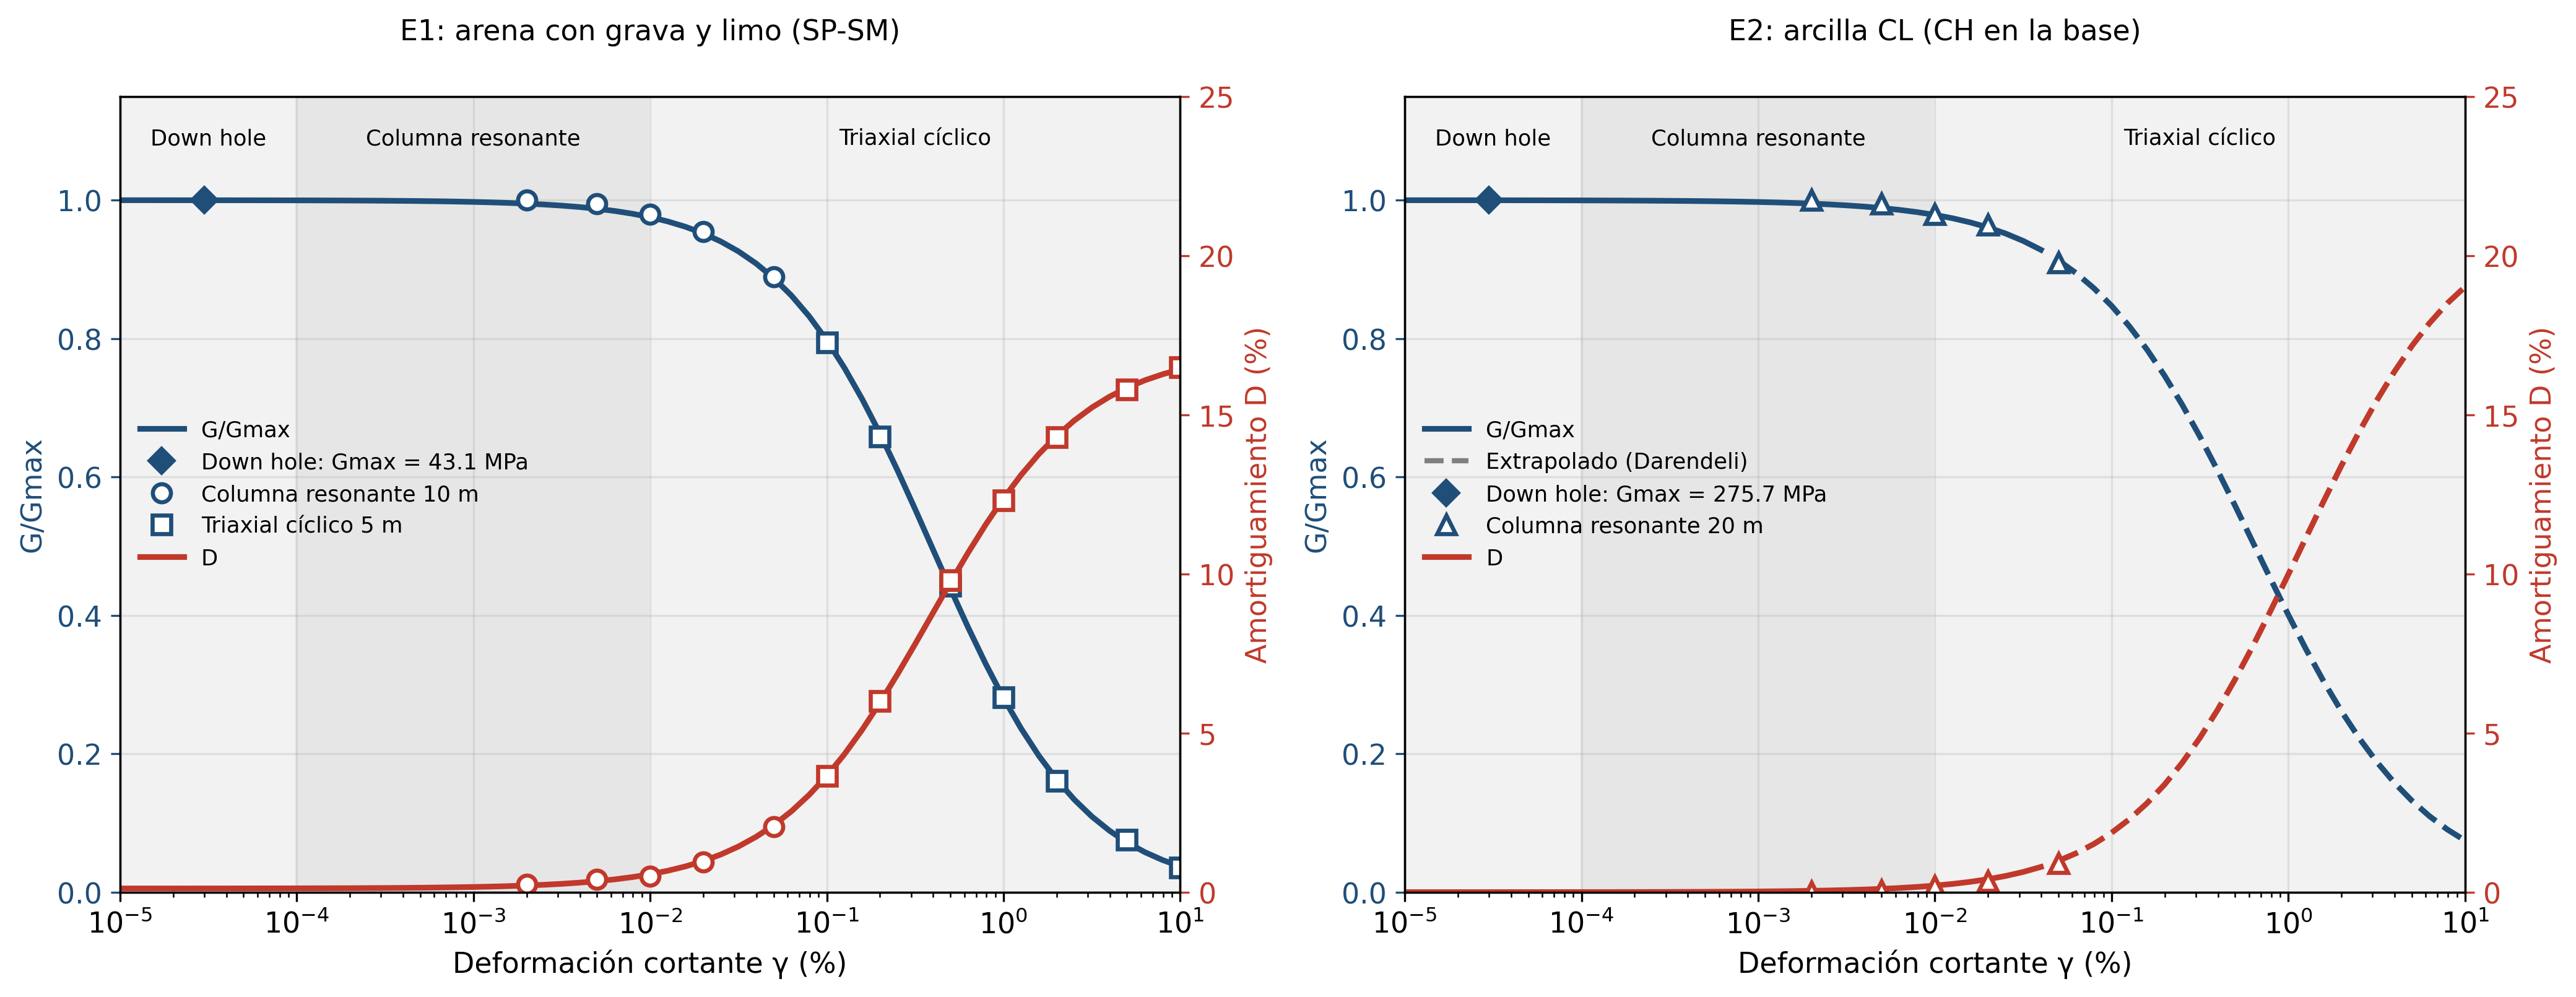
\includegraphics[width=\linewidth]{../figuras/curvas_degradacion_estratos.png}
    \caption{Curvas de degradación y amortiguamiento por estrato.}
    \label{fig:curvas}
\end{figure}

La curva de la arena se ajusta bien a los puntos de los ensayos
($R^2=0.9999$). Los dos suelos se degradan menos de lo que predice el modelo
de Darendeli; esto puede deberse a que las muestras se ensayaron con más
confinamiento que el que tienen en campo, por lo que en el sitio las curvas
podrían caer un poco antes.
\pendiente{Nota para el punto 5 (DEEPSOIL): la curva de la arcilla (E2)
solo tiene datos hasta $\gamma=0.05\%$ (columna resonante de 20 m); el resto
(línea punteada) se completó por ahora con la forma del modelo de Darendeli
($a=0.919$, $\gamma_r=0.65\%$) ajustada a esos puntos. La idea es reemplazarla,
como en el trabajo de referencia, por la curva de Vucetic y Dobry (1991) que
trae DEEPSOIL: probar IP $=15$ y IP $=30$ (la arcilla tiene IP $\approx18$),
compararlas con los 5 puntos de la columna resonante (Tabla~\ref{tab:dinE2}) y
escoger la que mejor se ajuste. Al cambiarla hay que actualizar la
Figura~\ref{fig:curvas}, la Tabla~\ref{tab:curvas} y este texto. Revisar
también $D_{\min}$ de la arcilla: el ajuste dio 0\% porque el ensayo mide
0.02\% a $\gamma=0.002\%$, muy bajo para DEEPSOIL (valores usuales de 0.5 a
2\%; la referencia usó 5\% en todas las capas). La arena (E1) no necesita
cambios: su curva sale completa de los ensayos.}

\section{Punto 3: análisis modal de Zeevaert}

\pendiente{Desplazamientos y $G$ contra profundidad por el método modal de
\textcite{zeevaert1983}.}

\section{Punto 4: sismos de análisis}

\pendiente{Tres registros de fuente cercana, intermedia y lejana. Propuesta:
ligarlos a la desagregación de la Entrega 2 (sismo cortical de
$M_w\approx6.0$ a unos 33 km y sismo intraplaca de $M_w\approx6.9$ a unos
130 km) y usar los registros del PEER de la Entrega 1.}

\section{Punto 5: análisis en DEEPSOIL}

\pendiente{Desplazamientos y $G$ contra profundidad con DEEPSOIL y
comparación con Zeevaert.}

\section{Punto 6: espectro de aceleración en superficie}

\pendiente{Espectro en superficie de DEEPSOIL comparado con el de la NSR-10
para perfil tipo D.}

\section{Punto 7: potencial de licuación}

\pendiente{Potencial de licuación con el nivel freático en superficie, con
Zeevaert y con DEEPSOIL. El estrato E1 (arena suelta saturada, $V_s$ de 143
a 160 m/s) es el de mayor interés; métodos de referencia:
\textcite{seed1971} y \textcite{youd2001}.}

\section{Conclusiones}

\pendiente{Conclusiones en viñetas.}

\section*{Referencias}
\small
\printbibliography[heading=none]

\end{document}
